\section{Methods}
\label{sec:methods}

\subsection{Dataset}
This consists of images, their descriptions and the textual context in which these images occur. Many datasets, such as ImageNET \cite{Russakovsky2012} and MSCOCO \cite{Lin2014}, exist of which many only consist of images and their description. Though, next to images and their annotations, in this approach the dataset also needs to include the context in which the image is in. In the literature the MSCOCO and/or Flickr8K/Flickr30K dataset are used for various image retrieval tasks as well as for image annotation tasks. In order to compare the models in the literature with the model in the thesis and since this dataset contains the required components to develop and train a model for automatic image description generation, either one of these datasets can be used. 

However, the textual context still is lacking in either of these datasets. Another dataset -- ImageCLEF \cite{Gilbert15_CLEF}, consisting of 500,000 images  from various sources on the internet -- does have some representation of textual context, since this dataset also contains the webpages on which the images are hosted. This can be used as the context for the images.

Since the literature mainly uses MSCOCO and/or the Flickr datasets and the results of this thesis has to be compared to earlier research, the MSCOCO dataset is used. This dataset is constructed with photos from the Flickr website. However, only the direct link to the photo is provided. Therefore, the Flickr API is used to retrieve the title and the description provided by the author of the photo.

However, the model of this thesis will be used by Dedicon and data that they have might not represent the data that is used by MSCOCO. First of all the language (English vs. Dutch) is different which will have a big impact if this model were to be trained on the MSCOCO dataset and then tested on the Dedicon dataset. Furthermore, the images in the Dedicon dataset might be of an entirely different category compared with the images in the MSCOCO dataset. Therefore, only one of the datasets can be used to both train and test the model on. Once a working prototype of the model has been created and trained, the model is tested on a subset of the dataset that is used. 

\subsection{Experimental setup}
The specifications of the computer that is used during the experiments are as follows: NVIDIA Quadro K2200 GPU with 4GB GDDR5 memory, 16 core Intel Xeon E5-1660 3Ghz CPU and 32GB of RAM.
% TODO: Additional information

\subsection{Image pre-processing}
Regularly words in a description correspond with a region in the image. This information can be used to improve the novel description generation of images. A first step in pre-processing would be to localize objects in the image which then result in bounding-boxes that describe regions of interest. Of the state-of-the-art methods that recognize objects -- such as exhaustive search \cite{zhu2010latent, felzenszwalb2010object} and selective search \cite{Sande2011} -- selective search by \citeauthor{Sande2011} repurposes segmentation for object recognition. Selective search is a much faster method that prefers approximate over exact object localization, has a high recall and permits the use of more expensive features such as bag-of-words. With this method several candidate bounding boxes are generated per image.  

The next step is using these candidates as an input for a Regional Convolutional Neural Network (R-CNN) \cite{girshick2015fast}. In essence, the purpose of the R-CNN is to score each candidate using a localization CNN which is pre-trained on the ImageNet dataset. The network receives two inputs: a batch of images and a list of regions of interest. The output of the network is a class posterior probability distribution and bounding-box offsets relative to the candidates. 

For the CNN the three best networks -- ordered from smallest to largest -- are the CaffeNet network \cite{Girshick2014} (equivalent to the AlexNet network), the VGG-CNN-M-1024 network \cite{chatfield2014return} and the VGG16 network \cite{simonyan2014very}. Due to hardware limitations, the third network was not able to be loaded into the GPU memory. Therefore, the second network is used instead which differs in width compared to CaffeNet.
The R-CNN is trained on the 81 classes that are included in the MSCOCO dataset using the VGG-CNN-M-1024 network.

The result of the image pre-processing step are the top 19 detected regions of interest in addition to the whole image. Thus, the representation of an image in bounding box $b$ is:

\begin{equation}
	r_i = CNN(I_b)
\end{equation}

where the CNN converts the sub-image $I_b$ into a 4096-dimensional feature vector.

The image pre-processing pipeline is depicted in Figure~\ref{fig:image-preprocessing}.

\begin{figure}
\centering  

\tikzstyle{input} = [coordinate]
\tikzstyle{combine} = [draw, fill=blue!20, circle]
\tikzstyle{method} = [draw, fill=blue!20, rectangle, 
    minimum height=3em, minimum width=6em]
    
\begin{tikzpicture}[auto, node distance=4.5cm,>=latex']
	% image stack
	\node at 	(0.4,0.5) {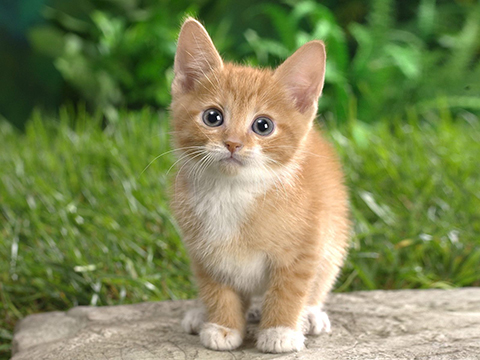
\includegraphics[width=0.04\textwidth]{images/cat}};

	\node [input, name=input] {};
	\node [combine, right of=input, node distance=1cm] (inputnode) {};
	\node [method, right of=inputnode, node distance=2.5cm]	 (selectivesearch) {selective search};
	\node [method, right of=selectivesearch, node distance=5cm] (rcnn) {R-CNN};
	\node [combine, below of=inputnode, node distance=2cm] (bbox) {};
	\node [method, below of=bbox, node distance=2cm] (cnn) {CNN};
	
	\draw [draw,->] (input) -- node {} (inputnode);
	\draw [->] (inputnode) -- node {$i$} (selectivesearch);
	\draw [->] (selectivesearch) -- node {candidates} (rcnn);
	\draw [->] (rcnn) |- node {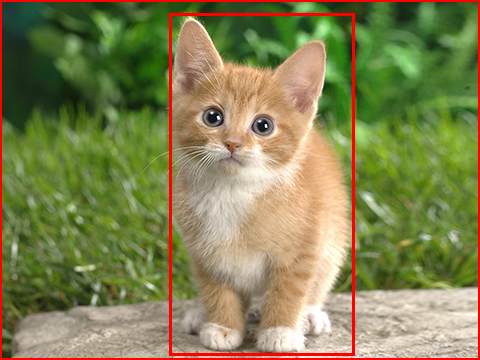
\includegraphics[width=0.1\textwidth]{images/catbb}} (bbox);
	\draw [->] (inputnode) -- node{$i$} (bbox);
	%\draw (inputnode) edge[out=90, in=90, distance=2cm, below, ->] node {$i$} (bbox);
	\draw [->] (bbox) -- node {regions} (cnn);
\end{tikzpicture}
\caption{Image pre-processing pipeline. Each image $i\in I$ is processed (in batches or individually) by this pipeline resulting in regions of interest in each image.}
\label{fig:image-preprocessing}
\end{figure}

\subsection{Sentence pre-processing}
